\documentclass[conference]{IEEEtran}

% -----------------------------------------------------------------------------
% Pacotes
% -----------------------------------------------------------------------------
\usepackage[utf8]{inputenc}
\usepackage[T1]{fontenc}
\usepackage[brazil]{babel}
\usepackage{graphicx}
\usepackage{booktabs}
\usepackage{amsmath}
\usepackage{siunitx}
\usepackage{listings}
\usepackage{pgfplots}
\usepackage{hyperref}
\usepackage{xcolor}
\usepackage{microtype}

\pgfplotsset{compat=1.18}
\usepgfplotslibrary{groupplots}
\graphicspath{{figures/}}

\hypersetup{
    colorlinks=true,
    linkcolor=black,
    citecolor=black,
    urlcolor=black
}

\lstset{
    basicstyle=\ttfamily\footnotesize,
    breaklines=true,
    frame=single,
    columns=fullflexible,
    keepspaces=true,
    showstringspaces=false
}

\title{Exploração de Scan Chain e ATPG em um Módulo \texttt{stream\_merge} Parametrizável}

\author{
\IEEEauthorblockN{Pedro Henrique de Ros, Douglas Cavalheiro Carvalho e Matheus Susin Timmers}
\IEEEauthorblockA{
98G10-04 -- Confiabilidade e Segurança de Hardware\\
Pontifícia Universidade Católica do Rio Grande do Sul -- PUCRS\\
Professor: Anderson Domingues
}
}

\begin{document}
\maketitle

\begin{abstract}
Este trabalho explora técnicas de \textit{Design for Testability} (DfT), com ênfase em \textit{Scan Chain} e geração automática de padrões de teste (ATPG), utilizando as ferramentas Cadence Genus e Modus. Inicialmente, foi reproduzido o tutorial fornecido na disciplina, validando o fluxo completo de síntese, inserção de registradores de scan, geração de padrões e simulação. Em seguida, o mesmo fluxo foi adaptado ao módulo parametrizável \texttt{stream\_merge}, empregado no trabalho anterior da disciplina, e automatizado para permitir a exploração dos parâmetros \texttt{DATA\_W}, \texttt{DEPTH} e \texttt{WMAX}. No tutorial de referência foram observados 116 registradores escaneáveis, duas cadeias de scan e cobertura ATPG de 99,97\%. Para a configuração padrão do \texttt{stream\_merge} ($32/8/7$), foram obtidos 298 registradores de scan, 100\% de registradores escaneáveis, uma cadeia de scan, cobertura ATPG de 99,99\% e simulação full-scan com 47 de 47 testes aprovados. A exploração de sete configurações mostrou que \texttt{DATA\_W} e \texttt{DEPTH} exercem influência dominante sobre a quantidade de registradores de scan e sobre a área, enquanto \texttt{WMAX} apresenta impacto reduzido. O overhead de área após DfT variou de 16,96\% a 20,14\%, enquanto a cobertura ATPG permaneceu entre 99,98\% e 99,99\% em todos os casos avaliados.
\end{abstract}

\begin{IEEEkeywords}
Design for Testability, DfT, Scan Chain, ATPG, Genus, Modus, síntese lógica, cobertura de teste.
\end{IEEEkeywords}

% -----------------------------------------------------------------------------
\section{Introdução}
% -----------------------------------------------------------------------------
A testabilidade de circuitos digitais é um aspecto importante do fluxo de desenvolvimento de hardware, principalmente quando o objetivo é detectar falhas estruturais em circuitos sequenciais. Técnicas de \textit{Design for Testability} (DfT) modificam ou complementam a estrutura do circuito para aumentar a controlabilidade e a observabilidade de nós internos durante o teste. Entre essas técnicas, o teste estrutural por \textit{scan} substitui elementos de estado convencionais por células compatíveis com scan e conecta esses elementos em uma ou mais cadeias serializáveis \cite{ensilica_dft}.

O Trabalho T2 da disciplina propõe a reprodução de um tutorial com Cadence Genus e Modus e, posteriormente, a adaptação desse fluxo ao módulo parametrizável \texttt{stream\_merge}. O enunciado também solicita a geração e execução de padrões de teste com automação, a exploração dos parâmetros do módulo, relatórios de área e potência e a análise da cobertura de teste para diferentes configurações \cite{enunciado_t2}.

Neste trabalho, além de reproduzir o fluxo fornecido, foi desenvolvido um processo automatizado para sintetizar, inserir DfT, preservar os artefatos de ATPG, executar o Modus e consolidar os resultados. A análise experimental foi organizada de modo a variar um parâmetro por vez em torno da configuração padrão, permitindo observar separadamente o impacto de \texttt{DATA\_W}, \texttt{DEPTH} e \texttt{WMAX}.

% -----------------------------------------------------------------------------
\section{Fundamentação}
% -----------------------------------------------------------------------------
\subsection{Scan Chain e DfT}

No teste estrutural por scan, registradores funcionais são substituídos por células que podem operar em dois modos. No modo funcional, o circuito preserva o comportamento original. No modo de teste, os registradores são conectados em cadeia e passam a funcionar como um registrador de deslocamento, permitindo inserir estados internos e observar respostas de forma serial. Essa transformação aumenta a controlabilidade e a observabilidade dos elementos sequenciais \cite{ensilica_dft}.

A inserção de DfT apresenta custos associados. Entre eles estão o aumento de área de silício, possíveis impactos de desempenho e potência e a necessidade de recursos adicionais de projeto e teste \cite{ensilica_dft}. Por esse motivo, a exploração paramétrica realizada neste trabalho considera não apenas a cobertura ATPG, mas também a área e a potência reportadas pelo Genus antes e depois da inserção de scan.

\subsection{ATPG}

Após a construção das cadeias de scan, a ferramenta ATPG utiliza o modelo estrutural do circuito para gerar padrões capazes de detectar falhas no modelo adotado. Neste trabalho, o Cadence Modus foi empregado para construção do modelo lógico, construção e verificação do modo \texttt{FULLSCAN}, criação do modelo de falhas, geração dos testes, escrita dos vetores e consolidação dos padrões. A cobertura ATPG foi utilizada como métrica para avaliar a efetividade do espaço de teste entre diferentes parametrizações do \texttt{stream\_merge}.

% -----------------------------------------------------------------------------
\section{Metodologia}
% -----------------------------------------------------------------------------
\subsection{Reprodução do tutorial}

O fluxo inicial utilizou o projeto \texttt{busca\_padrao} fornecido no tutorial. A sequência de síntese no Genus foi composta por leitura do RTL e das restrições, seguida dos comandos \texttt{syn\_generic}, \texttt{syn\_map} e \texttt{syn\_opt}. Em seguida, o script \texttt{dft\_setup.tcl} configurou o estilo \texttt{muxed\_scan}, identificou sinais de teste, verificou regras DfT, substituiu os flip-flops por células de scan e conectou automaticamente as cadeias.

O script fornecido mantém separados os registradores acionados em bordas positiva e negativa do mesmo clock. Como consequência, no tutorial foram obtidas duas cadeias: uma com 100 registradores e outra com 16, totalizando 116 registradores escaneáveis. Após a inserção de scan, foram exportados o \textit{scan definition}, o arquivo STIL e os arquivos necessários ao ATPG no Modus.

\subsection{Adaptação ao \texttt{stream\_merge}}

O módulo analisado recebe dois fluxos de pacotes \textit{valid/ready} e os combina em uma única saída através de uma FIFO interna. A arbitragem de entrada é ponderada e preserva a atomicidade dos pacotes, de modo que um pacote iniciado em uma entrada deve ser concluído antes que a arbitragem possa trocar de fonte \cite{enunciado_t2}.

A configuração padrão definida no enunciado é:
\begin{equation}
\texttt{DATA\_W}=32, \qquad \texttt{DEPTH}=8, \qquad \texttt{WMAX}=7.
\end{equation}
O parâmetro \texttt{DEPTH} deve ser potência de dois e maior ou igual a 2, enquanto \texttt{WMAX} deve ser maior ou igual a 1 \cite{enunciado_t2}.

As restrições de síntese utilizadas na adaptação definiram um clock \texttt{clk} com período de \SI{2.0}{\nano\second}, caminho falso a partir de \texttt{rst\_n}, atraso máximo de entrada de \SI{0.2}{\nano\second}, além das transições de entrada e cargas de saída utilizadas no fluxo original. O projeto foi sintetizado com Genus 21.12-s068\_1 e o ATPG foi executado com Modus 21.10-p003\_1. A simulação dos padrões full-scan utilizou Xcelium.

\subsection{Automação}

Para permitir a exploração de múltiplas configurações, o fluxo foi parametrizado utilizando a opção \texttt{-parameters} do comando \texttt{elaborate}. Um trecho representativo do script é apresentado a seguir.

\begin{lstlisting}
set TAG "DATA_W${DATA_W}_DEPTH${DEPTH}_WMAX${WMAX}"

read_hdl -sv stream_merge.sv
elaborate -parameters [list \
    [list DATA_W $DATA_W] \
    [list DEPTH  $DEPTH]  \
    [list WMAX   $WMAX]] $DESIGN

read_sdc ./constraint/stream_merge.sdc
syn_generic
syn_map
syn_opt

report_area > $RESULTDIR/area_pre_dft.rpt
report_power -unit mW > $RESULTDIR/power_pre_dft.rpt

include dft_setup.tcl

report_area > $RESULTDIR/area_post_dft.rpt
report_power -unit mW > $RESULTDIR/power_post_dft.rpt
\end{lstlisting}

Além da automação do Genus, scripts em \textit{shell} e Python foram utilizados para executar as configurações, preservar os arquivos gerados para o Modus, consolidar área, potência e quantidade de registradores scan e extrair a cobertura ATPG. Durante a execução em lote, o ambiente do Modus apresentou falhas intermitentes de inicialização ao usar o fluxo baseado em arquivo Tcl. Para contornar essa instabilidade, os comandos ATPG foram enviados diretamente à interface Tcl do Modus e foi implementado um mecanismo de repetição para os casos que apresentaram falha de inicialização. Esse ajuste não alterou o circuito nem os padrões gerados; apenas tornou a execução automatizada mais robusta.

\subsection{Planejamento experimental}

A exploração foi feita variando um parâmetro por vez em torno do caso padrão $32/8/7$. Foram avaliadas sete configurações únicas:
\begin{itemize}
    \item \texttt{DATA\_W}: 16, 32 e 64, mantendo \texttt{DEPTH}=8 e \texttt{WMAX}=7;
    \item \texttt{DEPTH}: 4, 8 e 16, mantendo \texttt{DATA\_W}=32 e \texttt{WMAX}=7;
    \item \texttt{WMAX}: 3, 7 e 15, mantendo \texttt{DATA\_W}=32 e \texttt{DEPTH}=8.
\end{itemize}

Para cada configuração foram coletados: número de células antes e depois de DfT, área total, potência total, overhead de área e potência, número de cadeias, número de registradores scan, quantidade de testes ATPG, cobertura ATPG/global e falhas não testadas.

% -----------------------------------------------------------------------------
\section{Resultados}
% -----------------------------------------------------------------------------
\subsection{Tutorial de referência}

A síntese do \texttt{busca\_padrao} resultou em 706 células e área total de 5290,415 nas unidades reportadas pelo Genus. A verificação DfT identificou zero violações e 116 registradores escaneáveis, correspondendo a 100\% dos registradores do projeto. Como o tutorial possuía registradores acionados em borda positiva e negativa, foram criadas duas cadeias de scan, de comprimentos 100 e 16, respectivamente.

\begin{figure*}[!t]
    \centering
    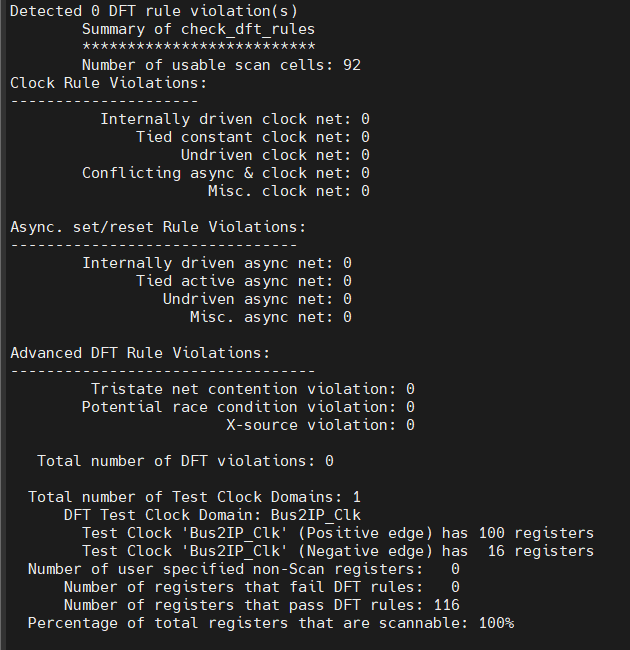
\includegraphics[width=0.47\textwidth]{tutorial_dft_rules.png}
    \hfill
    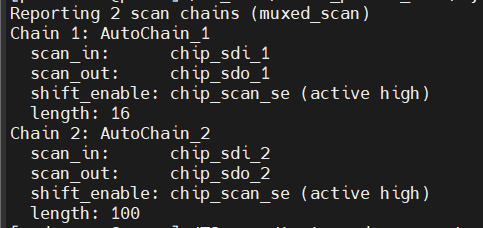
\includegraphics[width=0.47\textwidth]{tutorial_scan_chains.png}
    \caption{Validação DfT do tutorial. À esquerda, zero violações e 116 registradores 100\% escaneáveis. À direita, duas cadeias de scan com comprimentos 16 e 100.}
    \label{fig:tutorial_dft}
\end{figure*}

A geração ATPG atingiu 99,97\% de cobertura, com 415 testes simulados, 408 testes efetivos e duas falhas remanescentes no resumo final do Modus. Na simulação full-scan foram executados 410 testes, todos aprovados, totalizando 52048 comparações sem \textit{miscompares}.

\begin{figure*}[!t]
    \centering
    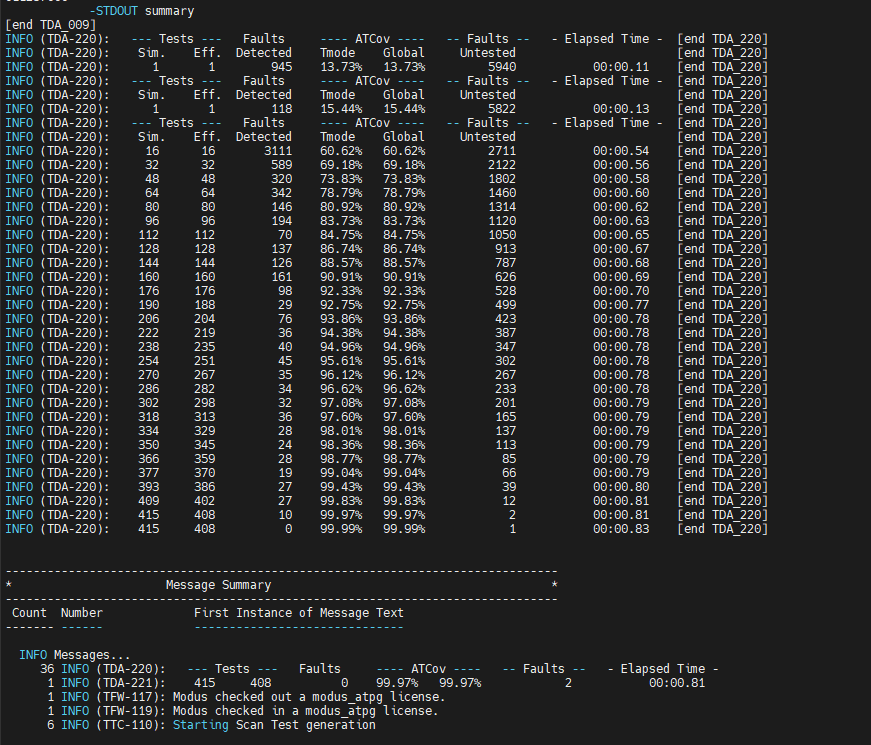
\includegraphics[width=0.47\textwidth]{tutorial_atpg.png}
    \hfill
    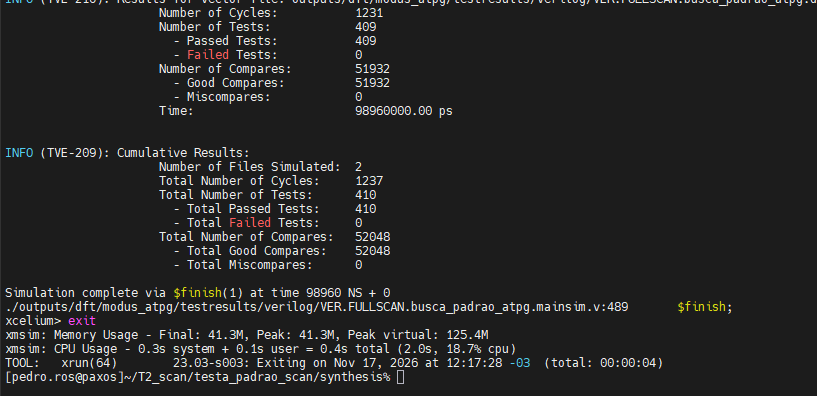
\includegraphics[width=0.47\textwidth]{tutorial_fullscan.png}
    \caption{Resultados do tutorial. À esquerda, evolução e resumo da cobertura ATPG; à direita, simulação full-scan com 410 testes aprovados e zero \textit{miscompares}.}
    \label{fig:tutorial_atpg}
\end{figure*}

\subsection{Caso padrão do \texttt{stream\_merge}}

Na configuração padrão $32/8/7$, a síntese pré-DFT apresentou 581 células e área total de 6034,880. Após a inserção de scan, foram obtidas 584 células e área total de 7186,277, correspondendo a overhead de 19,08\%. A potência reportada passou de \SI{3.84396}{\milli\watt} para \SI{3.86765}{\milli\watt}, variação de 0,62\%.

A verificação DfT não encontrou violações. Todos os 298 registradores passaram as regras DfT e foram considerados escaneáveis. Diferentemente do tutorial, o \texttt{stream\_merge} utiliza somente registradores de borda positiva no domínio de clock avaliado; por isso, a criação automática resultou em uma única cadeia com 298 elementos.

\begin{figure*}[!t]
    \centering
    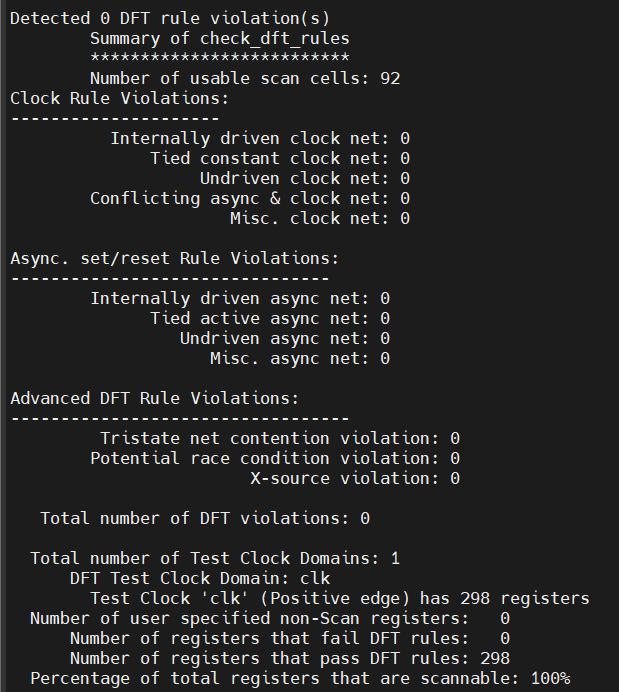
\includegraphics[width=0.47\textwidth]{stream_dft_rules.png}
    \hfill
    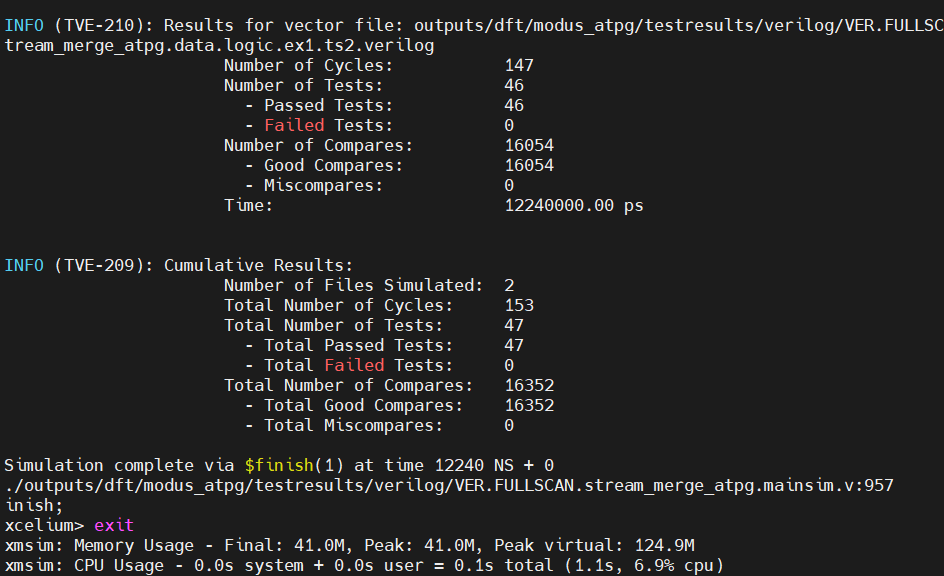
\includegraphics[width=0.47\textwidth]{stream_fullscan.png}
    \caption{Caso padrão do \texttt{stream\_merge}. À esquerda, 298 registradores 100\% escaneáveis e zero violações DfT. À direita, simulação full-scan acumulada com 47 de 47 testes aprovados e zero \textit{miscompares}.}
    \label{fig:stream_default}
\end{figure*}

O ATPG do caso padrão atingiu 99,99\% de cobertura, com 46 testes efetivos e nenhuma falha não testada. A simulação dos vetores produzidos pelo Modus processou dois arquivos, totalizando 47 testes e 16352 comparações, todas corretas. A diferença entre 46 testes efetivos no resumo ATPG e 47 testes acumulados na simulação decorre da forma como os arquivos de vetores são contabilizados em cada etapa do fluxo.

\subsection{Exploração paramétrica}

A Tabela~\ref{tab:all_results} consolida as sete configurações sintetizadas. A área é apresentada nas unidades fornecidas pelo \texttt{report\_area} do Genus, enquanto a potência é expressa em mW.

\begin{table*}[!t]
\caption{Resultados consolidados da exploração paramétrica.}
\label{tab:all_results}
\centering
\scriptsize
\resizebox{\textwidth}{!}{%
\begin{tabular}{ccccrrrrrrrrr}
\toprule
\texttt{DATA\_W} & \texttt{DEPTH} & \texttt{WMAX} & Scan regs. & Área pré & Área pós & OH área (\%) & Pot. pré (mW) & Pot. pós (mW) & OH pot. (\%) & Testes efet. & ATPG (\%) & Falhas não test. \\
\midrule
16 & 8  & 7  & 170 & 3621,488  & 4289,085  & 18,43 & 2,37676 & 2,38707 &  0,43 & 47 & 99,99 & 0 \\
32 & 4  & 7  & 155 & 3542,543  & 4143,488  & 16,96 & 2,60735 & 2,63689 &  1,13 & 34 & 99,99 & 0 \\
32 & 8  & 3  & 296 & 5975,422  & 7115,332  & 19,08 & 3,65515 & 3,66801 &  0,35 & 48 & 99,98 & 1 \\
32 & 8  & 7  & 298 & 6034,880  & 7186,277  & 19,08 & 3,84396 & 3,86765 &  0,62 & 46 & 99,99 & 0 \\
32 & 8  & 15 & 300 & 6119,472  & 7278,917  & 18,95 & 3,93459 & 3,97247 &  0,96 & 43 & 99,99 & 0 \\
32 & 16 & 7  & 581 & 11196,465 & 13451,840 & 20,14 & 5,31704 & 5,32096 &  0,07 & 77 & 99,99 & 0 \\
64 & 8  & 7  & 554 & 10807,504 & 12950,883 & 19,83 & 6,60105 & 6,43792 & -2,47 & 50 & 99,99 & 0 \\
\bottomrule
\end{tabular}%
}
\end{table*}

\subsubsection{Quantidade de registradores scan}

A Fig.~\ref{fig:scan_sweeps} apresenta a quantidade de registradores scan em função de cada parâmetro. A influência de \texttt{DATA\_W} e \texttt{DEPTH} é significativamente maior que a de \texttt{WMAX}. Ao variar \texttt{DATA\_W} de 16 para 64, a quantidade de registradores aumenta de 170 para 554. Para \texttt{DEPTH}, a variação de 4 para 16 eleva o total de 155 para 581. Em contraste, a variação de \texttt{WMAX} de 3 para 15 altera o total apenas de 296 para 300.

Esse comportamento é coerente com a estrutura do módulo: \texttt{DATA\_W} define a largura dos dados armazenados na FIFO e \texttt{DEPTH} define a quantidade de posições de armazenamento. Já \texttt{WMAX} modifica principalmente a largura dos registradores de crédito, cujo peso relativo no total de estado do circuito é pequeno.

\begin{figure*}[!t]
\centering
\begin{tikzpicture}
\begin{groupplot}[
    group style={group size=3 by 1, horizontal sep=1.3cm},
    width=0.29\textwidth,
    height=0.22\textwidth,
    grid=major,
    mark size=2pt,
    tick label style={font=\scriptsize},
    label style={font=\scriptsize},
    title style={font=\small}
]
\nextgroupplot[title={Variação de \texttt{DATA\_W}}, xlabel={\texttt{DATA\_W}}, ylabel={Registradores scan}, xtick={16,32,64}]
\addplot+[mark=*] coordinates {(16,170) (32,298) (64,554)};

\nextgroupplot[title={Variação de \texttt{DEPTH}}, xlabel={\texttt{DEPTH}}, ylabel={Registradores scan}, xtick={4,8,16}]
\addplot+[mark=*] coordinates {(4,155) (8,298) (16,581)};

\nextgroupplot[title={Variação de \texttt{WMAX}}, xlabel={\texttt{WMAX}}, ylabel={Registradores scan}, xtick={3,7,15}]
\addplot+[mark=*] coordinates {(3,296) (7,298) (15,300)};
\end{groupplot}
\end{tikzpicture}
\caption{Quantidade de registradores scan em função dos parâmetros do \texttt{stream\_merge}. Em cada gráfico, os demais parâmetros permanecem no valor padrão.}
\label{fig:scan_sweeps}
\end{figure*}

\subsubsection{Área pré e pós-DFT}

A tendência observada para área acompanha a quantidade de estado do circuito. A Fig.~\ref{fig:area_sweeps} apresenta as curvas pré e pós-DFT. Para \texttt{DATA\_W}, a área pré-DFT cresce de 3621,488 para 10807,504 entre 16 e 64 bits; a área pós-DFT cresce de 4289,085 para 12950,883. Para \texttt{DEPTH}, o crescimento também é acentuado: de 3542,543 para 11196,465 antes de DfT e de 4143,488 para 13451,840 após DfT. A influência de \texttt{WMAX} é comparativamente pequena.

\begin{figure*}[!t]
\centering
\begin{tikzpicture}
\begin{groupplot}[
    group style={group size=3 by 1, horizontal sep=1.25cm},
    width=0.29\textwidth,
    height=0.22\textwidth,
    grid=major,
    mark size=2pt,
    tick label style={font=\scriptsize},
    label style={font=\scriptsize},
    title style={font=\small},
    legend style={font=\scriptsize}
]
\nextgroupplot[title={\texttt{DATA\_W}}, xlabel={\texttt{DATA\_W}}, ylabel={Área}, xtick={16,32,64}, legend pos=north west]
\addplot+[mark=*] coordinates {(16,3621.488) (32,6034.880) (64,10807.504)};
\addlegendentry{Pré-DFT}
\addplot+[mark=square*] coordinates {(16,4289.085) (32,7186.277) (64,12950.883)};
\addlegendentry{Pós-DFT}

\nextgroupplot[title={\texttt{DEPTH}}, xlabel={\texttt{DEPTH}}, ylabel={Área}, xtick={4,8,16}]
\addplot+[mark=*] coordinates {(4,3542.543) (8,6034.880) (16,11196.465)};
\addplot+[mark=square*] coordinates {(4,4143.488) (8,7186.277) (16,13451.840)};

\nextgroupplot[title={\texttt{WMAX}}, xlabel={\texttt{WMAX}}, ylabel={Área}, xtick={3,7,15}]
\addplot+[mark=*] coordinates {(3,5975.422) (7,6034.880) (15,6119.472)};
\addplot+[mark=square*] coordinates {(3,7115.332) (7,7186.277) (15,7278.917)};
\end{groupplot}
\end{tikzpicture}
\caption{Área pré e pós-DFT em função dos parâmetros. O overhead de scan permanece aproximadamente constante em termos percentuais, embora o valor absoluto cresça com o tamanho do circuito.}
\label{fig:area_sweeps}
\end{figure*}

O overhead de área ficou entre 16,96\% e 20,14\%, com média de aproximadamente 18,93\% nas sete configurações. Isso mostra que a inserção de scan produz um custo de área relevante e relativamente estável ao longo do espaço avaliado.

\subsubsection{Potência}

A potência pré-DFT aumentou principalmente com \texttt{DATA\_W} e \texttt{DEPTH}. O menor valor observado foi \SI{2.37676}{\milli\watt} para $16/8/7$, enquanto o maior foi \SI{6.60105}{\milli\watt} para $64/8/7$. A diferença entre os relatórios pré e pós-DFT foi pequena em comparação ao overhead de área, permanecendo entre $-2,47$\% e $+1,13$\%.

O caso $64/8/7$ apresentou potência pós-DFT menor que a pré-DFT. Como os valores utilizados são os resultados do \texttt{report\_power} padrão do fluxo de síntese, esse ponto é interpretado como efeito do remapeamento e da estimativa da ferramenta, e não como uma tendência de redução de potência causada pela inserção de scan. Assim, a conclusão mais consistente é que, no conjunto avaliado, o impacto de DfT sobre a estimativa de potência foi pequeno e não monotônico.

\subsection{Cobertura ATPG}

A cobertura permaneceu praticamente constante em todo o espaço experimental. Seis das sete configurações alcançaram 99,99\% de cobertura ATPG e global, sem falhas não testadas. O caso $32/8/3$ apresentou 99,98\% e uma única falha não testada. A quantidade de testes efetivos variou de 34 a 77, mostrando que o tamanho do conjunto de padrões não permanece constante mesmo quando a cobertura final é semelhante.

\begin{figure*}[!t]
\centering
\begin{tikzpicture}
\begin{axis}[
    width=0.88\textwidth,
    height=0.30\textwidth,
    ybar,
    ymin=99.95,
    ymax=100.00,
    ylabel={Cobertura ATPG (\%)},
    xlabel={Configuração \texttt{DATA\_W/DEPTH/WMAX}},
    symbolic x coords={16/8/7,32/4/7,32/8/3,32/8/7,32/8/15,32/16/7,64/8/7},
    xtick=data,
    x tick label style={rotate=25,anchor=east,font=\scriptsize},
    yticklabel style={font=\scriptsize},
    grid=major,
    nodes near coords,
    nodes near coords style={font=\scriptsize, /pgf/number format/fixed, /pgf/number format/precision=2}
]
\addplot coordinates {
    (16/8/7,99.99)
    (32/4/7,99.99)
    (32/8/3,99.98)
    (32/8/7,99.99)
    (32/8/15,99.99)
    (32/16/7,99.99)
    (64/8/7,99.99)
};
\end{axis}
\end{tikzpicture}
\caption{Cobertura ATPG para as sete configurações avaliadas. Todos os casos permaneceram acima de 99,98\%.}
\label{fig:coverage}
\end{figure*}

% -----------------------------------------------------------------------------
\section{Discussão}
% -----------------------------------------------------------------------------
Os resultados evidenciam três comportamentos principais. Primeiro, a quantidade de registradores scan cresce fortemente com parâmetros que aumentam diretamente o armazenamento do módulo. Esse efeito é especialmente claro em \texttt{DATA\_W} e \texttt{DEPTH}, pois a FIFO contém dados e bits de controle para cada posição. Como consequência, a área pré e pós-DFT segue tendência semelhante.

Segundo, o parâmetro \texttt{WMAX} possui impacto reduzido sobre o tamanho do circuito quando comparado aos demais. A variação de 3 para 15 aumentou a quantidade de registradores scan em apenas quatro elementos e elevou a área pré-DFT de 5975,422 para 6119,472. Isso é consistente com a função de \texttt{WMAX}, que altera a largura dos créditos da arbitragem, mas não a largura nem a quantidade de posições da FIFO.

Terceiro, a testabilidade estrutural permaneceu elevada em todo o espaço analisado. Mesmo com a quantidade de registradores scan variando de 155 a 581, a cobertura ficou entre 99,98\% e 99,99\%. Portanto, nas configurações estudadas, o aumento de complexidade do circuito elevou os custos físicos e, em alguns casos, a quantidade de padrões, mas não causou degradação significativa da cobertura ATPG.

A comparação com o tutorial também mostra uma diferença estrutural importante. O projeto de referência exigiu duas cadeias devido à presença de registradores em bordas diferentes do clock, enquanto todas as configurações do \texttt{stream\_merge} resultaram em uma única cadeia. A configuração padrão apresentou 298 registradores de scan, número superior aos 116 do tutorial, mas ainda assim obteve cobertura de 99,99\% e simulação full-scan sem falhas.

% -----------------------------------------------------------------------------
\section{Conclusões}
% -----------------------------------------------------------------------------
O trabalho reproduziu com sucesso o fluxo de DfT proposto no tutorial e o adaptou ao módulo \texttt{stream\_merge}. No tutorial, foram obtidos 116 registradores escaneáveis, duas cadeias de scan, cobertura ATPG de 99,97\% e simulação com 410 testes aprovados. Para o caso padrão do \texttt{stream\_merge}, foram obtidos 298 registradores escaneáveis, uma cadeia, zero violações DfT, cobertura ATPG de 99,99\% e 47 testes aprovados na simulação full-scan.

A automação desenvolvida permitiu explorar sete configurações do módulo e consolidar automaticamente relatórios de área, potência e cobertura. O estudo mostrou que \texttt{DATA\_W} e \texttt{DEPTH} dominam o crescimento de registradores scan e área, enquanto \texttt{WMAX} possui efeito reduzido. O overhead de área introduzido pelo scan permaneceu entre 16,96\% e 20,14\%, enquanto a cobertura ATPG permaneceu praticamente constante e superior a 99,98\% em todos os casos.

Dessa forma, a exploração demonstra que o custo físico da inserção de scan cresce com o tamanho do estado do circuito, porém a estratégia utilizada preservou alta testabilidade em todas as parametrizações avaliadas. Os scripts de automação e os arquivos necessários para reprodução do fluxo são disponibilizados no repositório público do trabalho, conforme solicitado no enunciado.

% -----------------------------------------------------------------------------
\begin{thebibliography}{00}

\bibitem{enunciado_t2}
A. Domingues, ``Trabalho T2 -- Scan Chain,'' disciplina 98G10-04 Confiabilidade e Segurança de Hardware, PUCRS, 2026.

\bibitem{ensilica_dft}
L. Rezende, ``Design for Testability,'' EnSilica plc, material de apoio da disciplina, 2023.

\end{thebibliography}

\end{document}
